\section{Auswertung}
\label{sec:Auswertung}
Die in \autoref{sec:Auswertung} gezeigten Grafiken und Rechnungen sind mithilfe der Python-Bibliotheken Matplotlib \cite{matplotlib}, Scipy \cite{scipy} und Numpy \cite{numpy}
erstellt worden. Die Fehlerrechnung wird mit der Python-Bibliothek Uncertainties \cite{uncertainties} durchgeführt.


\subsection{Überprüfung der Stabilitätsbedingung}
\label{sec:a1}
Die Stabilitätsbedingung, Gleichung \autoref{eqn:stab}, beschreibt den Bereich der Resonatorlänge des HeNe-LASERs, in dem der LASER-Strahl nicht divergiert.
Für die verwendeten Resonatoren aus Konkav-Konkav- und Plan-Konkav-Spiegelaufbauten ergeben sich mit einem Krümmungsradius von $r = \SI{1400}{mm}$ für die konkaven Spiegel die Stabilitätsgleichungen.
\begin{align}
  \left(g_1 \cdot g_2\right)_{\text{KK}} &= \left( 1 - \frac{L}{1400} \right)^2 \\
  \left(g_1 \cdot g_2\right)_{\text{PK}} &= 1 \cdot \left( 1 - \frac{L}{1400} \right) \, .
\end{align}
Diese erfüllen die Stabilitätsbedingungen für $0 \leq L \leq 2800 \, \, \mathrm{mm}$ für den bikonkaven Resonator und $0 \leq L \leq 1400 \, \, \mathrm{mm}$ für den Plan Konkaven Resonator.
\begin{figure}[H]
  \centering
  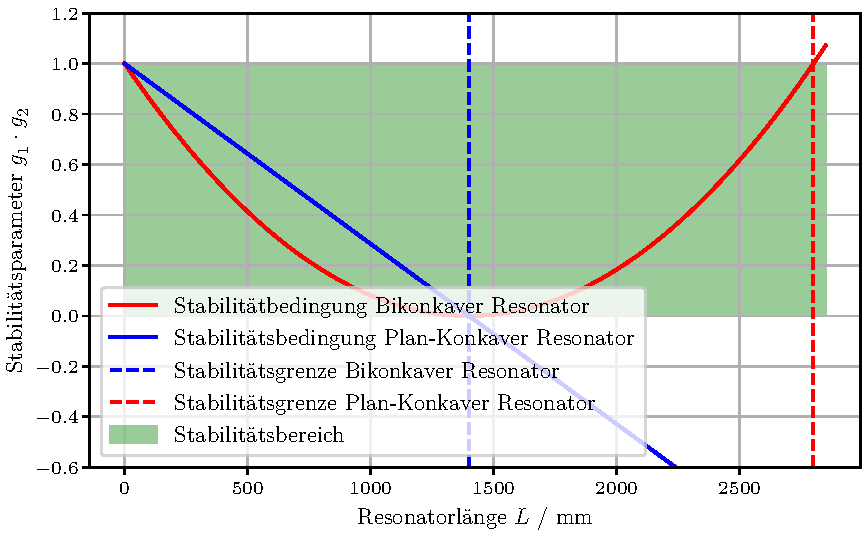
\includegraphics[width=0.7\linewidth]{plots/stab_theo.pdf}
  \caption{Theoretische Stabilitätsparameter für die verwendeten Resonatoren.}
  \label{fig:6}
\end{figure}
\noindent
In \autoref{fig:6} sind dabei die theoretischen Plots der Stabilitätsbedingung mit eingezeichneten Stabilitätsgrenzen zu sehen.
\begin{table}[H]
  \centering
  \caption{Messwerte der LASER Leistung als Funktion der Resonatorlänge, K-K Links und P-K Rechts.}
  \begin{tabular}{S[table-format=3] S[table-format=2(2)]}
      \toprule
      {$L$ / $\mathrm{cm}$} & {$P$ / $\mathrm{mW}$} \\
      \midrule
      45    &   6.99 \\
      50    &   6.33\\
      55    &   6.5\\
      60    &   4.89\\
      65    &   5.99\\
      70    &   4.23\\
      75    &   3.38\\
      80    &   5.17\\
      85    &   5.97\\
      90    &   6.4\\
      95    &   6.13\\
      100   &   4.23\\
      105   &   4.18\\
      110   &   4.87\\
      115   &   5.13\\
      120   &   4.65\\
      145   &   3.4\\
      \bottomrule
  \end{tabular}
  \begin{tabular}{S[table-format=3] S[table-format=2(2)]}
      \toprule
      {$L$ / $\mathrm{cm}$} & {$P$ / $\mathrm{mW}$} \\
      \midrule
      55.5 & 1.2\\
      70  & 0.57\\
      80 & 0.72\\
      90 & 2.14\\
      100 & 1.8\\
      110 & 0.7\\
      \\
      \\
      \\
      \\
      \\
      \\
      \\
      \\
      \\
      \\
      \\
      \bottomrule
  \end{tabular}
  \label{tab:1}
\end{table}
\noindent
In \autoref{tab:1} sind die Daten der Messreihe zur Verifizierung der Stabilitätsbedingung zu sehen. In diesen ist zu erkennen, dass der bikonkave Resonator auch bei Resonatorlängen über $\SI{1400}{mm}$ stabil funktioniert und der plankonkave Resonator ebenfalls in dem vorhergesagten Bereich funktioniert.
\begin{figure}[H]
  \centering
  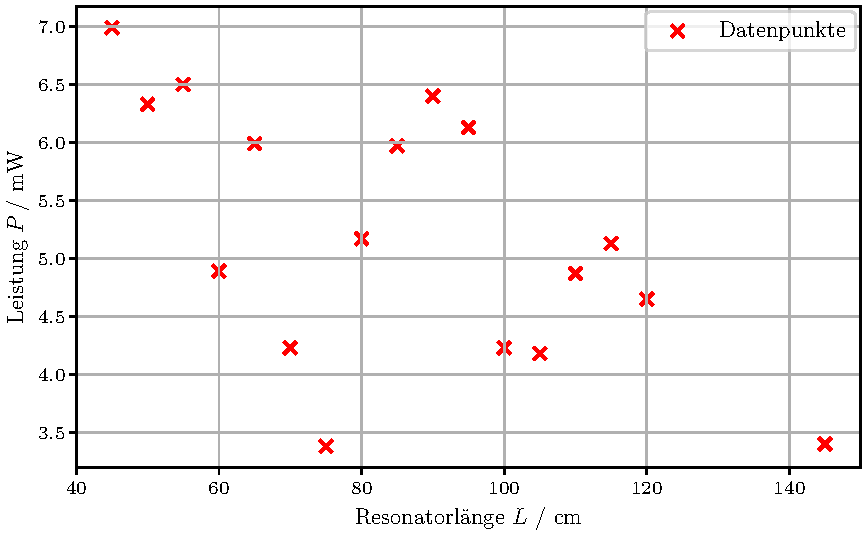
\includegraphics[width=0.65\linewidth]{plots/stab_bed_1.pdf}
  \caption{Leistung des LASERs als Funktion der Resonatorlänge}
  \label{fig:1}
\end{figure}
\noindent
Die Leistung des LASERs ist dabei unabhängig von der Länge des Resonators, wie in \autoref{fig:1} gut zu erkennen ist.
\newpage
\subsection{Messung der Wellenlänge des LASERs}
Für die Bestimmung der Wellenlänge wurden für vier verschiedene Gitter die Abstände der Beugungsmaxima vom Hauptmaximum gemessen, wie in \autoref{tab:3} zu sehen ist.
\begin{table}[H]
  \centering
  \caption{Abstände der Beugungsmaxima bei Gittern mit $g_1 = \SI{100}{\milli\meter}^{-1}$, $g_2 = \SI{80}{\milli\meter}^{-1}$, $g_3 = \SI{600}{\milli\meter}^{-1}$, $g_4 = \SI{1200}{\milli\meter}^{-1}$ (von links nach rechts).}
  \begin{tabular}{S[table-format=3] S[table-format=2(2)]}
      \toprule
      {$d_l$ / $\mathrm{cm}$} & {$d_r$ / $\mathrm{cm}$} \\
      \midrule
      4.2 & 4.2 \\
      7.6 & 7.6 \\
      11.7 & 11.5 \\
      16.2 & 15.3 \\
      20.9 & 19.2 \\
      25.8 & 23.4 \\
      31.5 & 27.9 \\
      37.9 & 32.7 \\
      \\
      \bottomrule
  \end{tabular}
  \begin{tabular}{S[table-format=3] S[table-format=2(2)]}
      \toprule
      {$d_l$ / $\mathrm{cm}$} & {$d_r$ / $\mathrm{cm}$} \\
      \midrule
      3.2 & 3 \\
      6.2 & 6 \\
      9.6 & 9 \\
      13 & 12.1 \\
      16.8 & 15.1 \\
      20.8 & 18.2 \\
      24.5 & 21.4 \\
      29.4 & 24.7 \\
      34.3 & 28.2 \\
      \bottomrule
  \end{tabular}
  \begin{tabular}{S[table-format=3] S[table-format=2(2)]}
    \toprule
    {$d_l$ / $\mathrm{cm}$} & {$d_r$ / $\mathrm{cm}$} \\
    \midrule
    12.4 & 12.2 \\
    36.1 & 34.1 \\
    \\
    \\
    \\
    \\
    \\
    \\
    \\
    \bottomrule
  \end{tabular}
  \begin{tabular}{S[table-format=3] S[table-format=2(2)]}
    \toprule
    {$d_l$ / $\mathrm{cm}$} & {$d_r$ / $\mathrm{cm}$} \\
    \midrule
    35.2 & 33.4 \\
    \\
    \\
    \\
    \\
    \\
    \\
    \\
    \\
    \bottomrule
  \end{tabular}
  \label{tab:3}
\end{table}
\noindent
Die Werte werden für jedes Gitter für jeweils jede Beugungsordnung links und rechts gemittelt und der Standardfehler des Mittelwerts gebildet, um für die Schiefe des Schirmes und des Gitters zur Strahlachse zu korrigieren.
Für jedes der Gitter wird dann in jeder Beugungsordnung nach \autoref{eqn:wel} die Wellenlänge berechnet und für jedes Gitter gemittelt. Es ergeben sich so für die gemessenen Wellenlängen für jedes Gitter auf
\begin{align}
  \label{eqn:2}
  \lambda_1 &= 641 \pm 11 \, \, \mathrm{nm} \, ,  \\
  \lambda_2 &= 640 \pm 10 \, \, \mathrm{nm} \, ,\\
  \lambda_3 &= 633 \pm 8 \, \, \mathrm{nm}  \, , \\
  \lambda_4 &= 627 \pm 11 \, \, \mathrm{nm} \, . \\
\end{align} 
Dabei ist die Reihenfolge der Gitter in der Wellenlängen Angabe in \autoref{eqn:2} identisch zu der in \autoref{tab:3} ist.
\newpage
\subsection{Messung der Polarisationsrichtung des LASERs}
In \autoref{tab:2} sind die Messwerte der Messreihe für die Bestimmung der Polarisationsrichtung des LASERs zu sehen.
\begin{table}[H]
  \centering
  \caption{Messwerte der Leistung des LASERs als Funktion des Polarisationswinkels.}
  \begin{tabular}{S[table-format=3] S[table-format=2(2)]}
      \toprule
      {Winkel $\Phi$ / $^\circ$} & {$P$ / $\mathrm{mW}$} \\
      \midrule
      0    &0.45 \\
      10   &0.96 \\
      20    &1.56 \\
      30    &2.15 \\
      40    &2.73 \\
      50    &3.13 \\
      60    &3.47 \\
      70    &3.58 \\
      80    &3.45 \\
      90    &3.07 \\
      100    &2.69 \\
      110    &2.06 \\
      120    &1.39 \\
      130    &0.82 \\
      140    &0.37 \\
      150    &0.1 \\
      160    &0.0 \\
      170    &0.13  \\
      \bottomrule
  \end{tabular}
  \begin{tabular}{S[table-format=3] S[table-format=2(2)]}
    \toprule
    {Winkel $\Phi$ / $^\circ$} & {$P$ / $\mathrm{mW}$} \\
    \midrule
    180    &0.45  \\
    190    &0.97 \\
    200    &1.54 \\
    210    &2.24 \\
    220    &2.77 \\
    230    &3.18 \\
    240    &3.5 \\
    250    &3.53 \\
    260    &3.37 \\
    270    &3.0 \\
    280    &2.66 \\
    290    &2.01 \\
    300    &1.39 \\
    310    &0.87 \\
    320    &0.37 \\
    330    &0.08 \\
    340    &0.0 \\
    350    &0.12 \\
    \bottomrule
  \end{tabular}
  \label{tab:2}
\end{table}
\noindent
Diese sind nach Gleichung (ref) proportional zu $\text{cos}^2\left(\Phi\right)$, wobei die Funktion maximal wird, wenn der Polarisationswinkel $\Phi_0$ erreicht ist. Dies ist durch eine Phasenverschiebung um diesen Winkel erreichbar, weswegen eine Funktion der Form
\begin{equation}
  \label{eqn:1}
  P\left(\Phi\right) = I_0 \cdot \text{cos}^2\left(\Phi - \Phi_0\right)
\end{equation}
in die Daten gefittet wurde.
\begin{figure}[H]
  \centering
  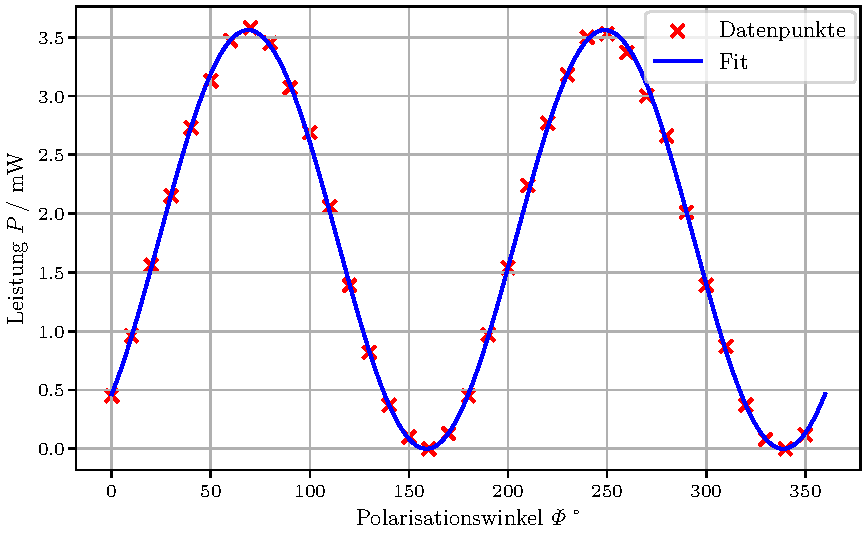
\includegraphics[width=0.7\linewidth]{plots/pol.pdf}
  \caption{Leistung des LASERs als Funktion des Polarisationswinkels.}
  \label{fig:2}
\end{figure}
\noindent
In \autoref{fig:2} sind die Daten in einem Scatter Plot aufgetragen und der zugehörige Fit der Funktion in \autoref{eqn:1} zu sehen.
Die Parameter der Gleichung lassen sich dabei auf
\begin{align}
  \Phi_0 &= 68.834 \pm 0.018 \, \, ^\circ \, ,\\
  I_0 &= 3.56078 \pm 0.00009 \, \, \mathrm{mW}
\end{align}
bestimmen, wobei $I_0$ die Leistung des Lasers ohne Polarisationsfilter ist.
\noindent
\newpage
\subsection{Abhängigkeit der longitudinalen Resonatormoden von der Resonatorlänge}
Wie in \autoref{sec:transversalemoden} beschrieben bilden sich im Resonator des LASERs longitudinale Moden aus, welche direkt von der Länge des Resonators abhängig sind. Die Frequenzen dieser Moden haben gleichmäßige Abstände, wie in \autoref{eqn:long} zu erkennen ist.
Ohne Fabry-Perot-Etalon ist der LASER im Multi-Moden-Betrieb und die longitudinalen Frequenzen und deren Abstände sind direkt messbar.
\begin{table}[H]
  \centering
  \caption{Position der longitudinalen Frequenz Peaks für verschiedene Resonatorlängen.}
  \begin{tabular}{S ||S| S| S| S| S| S}
      \toprule
      {\textbf{Resonatorlänge} / $\mathrm{cm}$} & {55.5} & {70}  & {80} & {90} & {100}  & {110}\\
      \midrule
      {\textbf{Pos. der Peaks} / $\mathrm{MHz}$} & 266 & 218& 188& 169& 154& 139\\
       &533 & 435 & 357 & 338 & 304 & 274 \\
       &799 & 653 & 563 & 506 & 454 & 409 \\
       &1065 & 818 & 746 & 675 & 608 & 544 \\
       & & &934 & 844 & 758 & 679 \\
       & & & &1013 & 908 & 814 \\
       & & & & 1181 & 1061 & \\
       & & & & 1350 & & \\
      \bottomrule
  \end{tabular}
  \label{tab:4}
\end{table}
\noindent
In \autoref{tab:4} sind die Messwerte dieser Peaks für verschiedene Resonatorlängen aufgetragen. Aus diesen Messwerten lassen sich die Abstände der Peaks, und durch das Umstellen der \autoref{eqn:long}, die zugehörige Resonatorlänge
\begin{equation}
  L = \frac{\text{c}}{2 \Delta \nu}
\end{equation}
berechnen. Ist \autoref{eqn:long} korrekt, so wird die Steigung einer Ausgleichsgeraden durch die berechneten Resonatorlängen gegen die tatsächlichen Resonatorlängen ca. 1 betragen.
\begin{figure}[H]
  \centering
  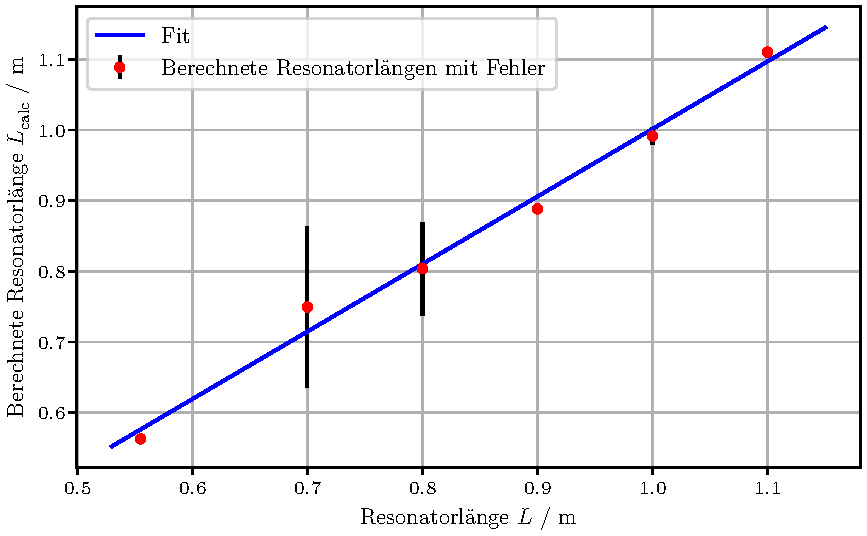
\includegraphics[width=0.7\linewidth]{plots/long_mode.pdf}
  \caption{Berechnete Resonatorlänge gegen die tatsächliche Resonatorlänge aufgetragen.}
  \label{fig:3}
\end{figure}
\noindent
In \autoref{fig:3} sind diese Darstellung und der zugehörige Fit zu sehen. Die Fitparameter der Geradengleichung
\begin{equation}
  f\left(x\right) = m \cdot x + n
\end{equation}
ergeben sich auf
\begin{align}
  m &= 0.956 \pm 0.003 \\
  n &= 0.046 \pm 0.002 \, \, \mathrm{m}
\end{align}
\newpage
\subsection{Messung der transversalen LASER Moden}
In Tabelle \ref{tab:5} sind die Messwerte der TEM Moden Vermessung abgebildet.
\begin{table}[H]
  \centering
  \caption{Leistung des LASERs $P$ für verschiedene Abstände von der Strahlachse $x$, links: $\text{TEM}_{00}$, rechts: $\text{TEM}_{01}$.}
  \begin{tabular}{S[table-format=3] S[table-format=2(2)]}
      \toprule
      {$x$ / $\mathrm{mm}$} & {$P$ / $\mathrm{mW}$} \\
      \midrule
      -8  & 0 \\
      -7  & 0.001\\
      -6  & 0.002\\
      -5  & 0.007\\
      -4  & 0.017\\
      -3  & 0.039\\
      -2  & 0.064\\
      -1  & 0.086\\
       0 & 0.095\\
       1 & 0.087\\
       2 & 0.06\\
       3 & 0.037\\
       4 & 0.018\\
       5 & 0.007\\
       6 & 0.002\\
       7 & 0.001\\
       8 & 0      \\
       \\
       \\
       \\
       \\
    \bottomrule
  \end{tabular}
  \begin{tabular}{S[table-format=3] S[table-format=2(2)]}
      \toprule
      {$x$ / $\mathrm{mm}$} & {$P$ / $\mathrm{mW}$} \\
      \midrule
      -10  & 0.0003   \\
      -9  & 0.0003 \\
      -8  & 0.0006 \\
      -7  & 0.002 \\
      -6  & 0.004 \\
      -5  & 0.009 \\
      -4  & 0.015 \\
      -3  & 0.022 \\
      -2  & 0.017 \\
      -1  & 0.003 \\
      0  & 0.0 \\
      1  & 0.011 \\
      2  & 0.016 \\
      3  & 0.017 \\
      4  & 0.014 \\
       5 & 0.01 \\
      6  & 0.003 \\
      7  & 0.0011 \\
      8  & 0.0003 \\
      9  & 0.0003 \\
     10 & 0.0004 \\
      \bottomrule
  \end{tabular}
  \label{tab:5}
\end{table}
\noindent
Wie im \autoref{sec:transversalemoden} der Theorie beschrieben, folgen die Intensitäten der $\text{TEM}_{lp}$ Moden den Hermite-Polynomen, überlagert mit einer Gaußverteilung.
Aufgrund dessen werden an die Daten der $\text{TEM}_{00}$ Messung eine Funktion der Form
\begin{equation}
  P\left(x\right) = I_0 \cdot \text{exp}\left( \frac{ -2 \left(x - x_1\right)^2}{\omega^2} \right)
\end{equation}
Und an die Daten der $TEM_{01}$ Messung eine Funktion der Form
\begin{equation}
  P\left(x\right) = I_0 \cdot \left(\frac{\left(x - x_1\right)}{\omega}\right)^2 \cdot \text{exp}\left( \frac{-2 \left(x - x_0\right)^2}{\omega^2} \right)
\end{equation}
gefittet. Dabei sind die Parameter $x_0$ und $x_1$ nicht Teil der Theorie, jedoch in den jeweiligen Fit-Funktionen, um für mögliche systematische Unsicherheiten zu korrigieren.
\begin{figure}[H]
    \centering
    \begin{minipage}{0.48\textwidth}
        \centering
        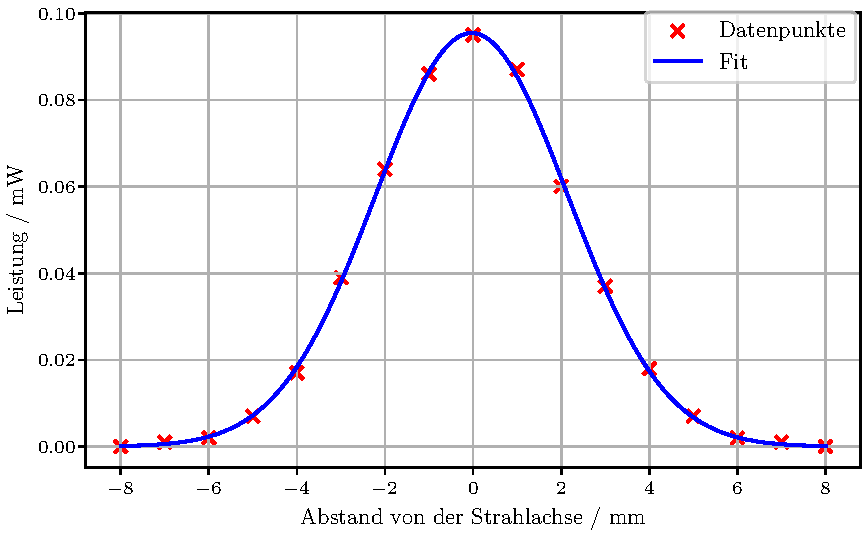
\includegraphics[width=1\textwidth]{plots/TEM_00.pdf}
        \caption{$TEM_{00}$ Daten und Fit.}
        \label{fig:4}
    \end{minipage}\hfill
    \begin{minipage}{0.48\textwidth}
        \centering
        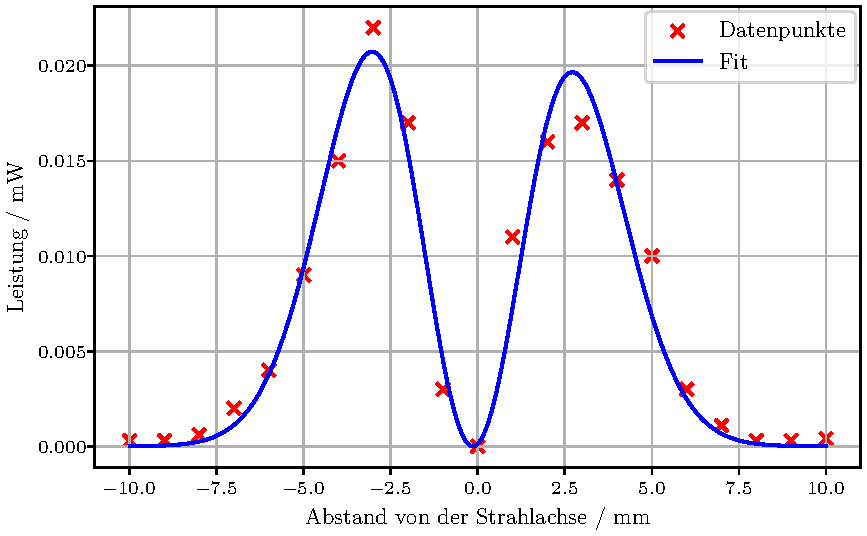
\includegraphics[width=1\textwidth]{plots/TEM_01.pdf}
        \caption{$TEM_{01}$ Daten und Fit.}
        \label{fig:5}
    \end{minipage}
\end{figure}
\noindent
In \autoref{fig:4} und \autoref{fig:5} sind die aufgetragenen Daten und zugehörigen Fits der beiden vermessenen TEM Moden zu sehen. Die Parameter des $\text{TEM}_{00}$ Fits ergeben sich dabei auf
\begin{align}
  I_0 &= 0.095 \pm 0.00 \, \, \mathrm{mW} \\
  x_1 &= -0.0322 \pm 0.0002 \, \, \mathrm{mm} \\
  \omega &= 4.3711 \pm 0.0009 \, \, \mathrm{mm}
\end{align}
und die Parameter der $\text{TEM}_{01}$ Mode auf
\begin{align}
  I_0 &= 0.11 \pm 0.00 \, \, \mathrm{mW} \\
  x_0 &= -0.139 \pm 0.005 \, \, \mathrm{mm} \\
  x_1 &= -0.178 \pm 0.005 \, \, \mathrm{mm} \\
  \omega &= 4.068 \pm 0.008 \, \, \mathrm{mm}
\end{align}
wobei die identischen Parameter $x_0$, $\omega$ und $I_0$ zwischen den Moden nur kleine Abweichungen voneinander aufweisen.
\newpage